\subsection{Convertidor CC-CC Conmutado}

Un convertidor CC-CC es un dispositivo electrónico que tiene como objetivo convertir una tensión continua, generalmente no regulada (es decir que no es fija), $V_{in}$ a la entrada, a una tensión continua regulada $V_{out}$ de distinta magnitud a la salida, transfiriendo la mayor cantidad de energía posible de la entrada hacia la salida. Dependiendo del tipo de convertidor, esta tensión de salida puede ser menor, mayor o tanto menor como mayor a la tensión de entrada.\\

Estos convertidores son de interés para nuestra aplicación, ya que la tensión $V_{stack}$ que entrega la pila (ecuación \ref{v_stack}) es una tensión continua no regulada, que varía apreciablemente con la corriente demandada; mientras que a la salida se demanda una tensión fija y regulada $V_{bus}$ para conectar al bus de continua del sistema híbrido de la figura \ref{SHGE}.\\

La forma más básica que se podría concebir para un dispositivo que cumpla esta función es la de un simple divisor resistivo, en el cual la tensión $V_{out}$ depende de las resistencias $R_1$ y $R_2$ y la tensión de entrada $V_{in}$.

\begin{equation*}
    V_{out} = V_{in}\cdot\frac{R_2}{R_1+R_2}
\end{equation*}

Entonces, variando la relación entre $R_1$ y $R_2$, se puede variar la tensión $V_{out}$ entre tensión nula y $V_{in}$. Sin embargo, se necesita solo un análisis superficial de esta topología para ver que no es viable para ningún tipo de aplicación, más que nada por su pobre eficiencia energética (para obtener una tensión igual a la mitad de la entrada, se pierde la mitad de la potencia en disipación resistiva).\\

Los convertidores CC-CC se suelen separar en dos principales categorías: los {\Medium reguladores lineales}, que son un caso complejizado del divisor resistivo donde se utiliza un transistor como resistencia varibale (además de un diodo para regular la tensión de salida); y los {\Medium convertidores conmutados}, en los cuales uno o más transistores, actuando como llaves, son conmutados a alta frecuencia y junto con dispositivos que almacenan energía (como inductores y capacitores) producen una tensión continua a la salida.\\

Dado que para esta plataforma se utiliza un convertidor conmutado (principalmente por su gran ventaja en eficiencia energética), se enfocará el análisis únicamente en éstos; comenzando por una explicación de los conceptos básicos necesarios para comprender su funcionamiento.\\

\subsubsection{Conceptos Básicos de Convertidores CC-CC Conmutados}

Como se detalló más arriba, los convertidores CC-CC conmutados consisten, en su forma más básica, en una fuente de continua no regulada a la entrada; y un transistor (que puede ser BJT, MOSFET o IGBT) que, mediante una excitación en su tercer terminal, se conmuta entre los modos de alta impedancia e impedancia nula, actuando como llave abierta y llave cerrada respectivamente. La proporción del tiempo total de ciclo ($T_s$) en la que el transistor está conduciendo ($t_{on}$) se denomina {\Medium ciclo de trabajo} o \textit{duty cycle} y se suele simbolizar con la letra $D$. Como se verá más adelante, este es un parámetro crucial para el funcionamiento de este tipo de convertidores, ya que controlándolo se puede variar el nivel de tensión y corriente de salida.

\begin{figure}[H]
    \centering
    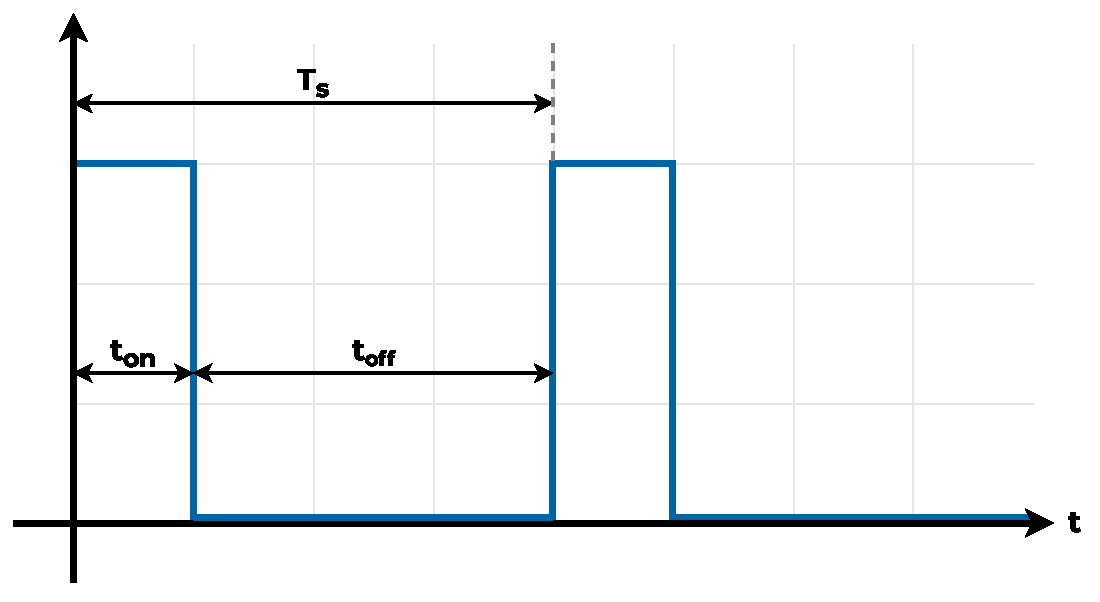
\includegraphics[scale=0.5]{Imagenes/Duty Cycle.pdf}
    \caption{Una forma de onda cuadrada con ciclo de trabajo $D$ del \SI{25}{\percent}.}
    \label{V-I_celda}
\end{figure}

Los convertidores CC-CC conmutados se clasifican en dos grandes grupos, usando como criterio la existencia de aislación galvánica entre la entrada no regulada y la salida regulada:

\begin{itemize}
    \item {\SemiBold Convertidores No Aislados:} son los convertidores que no tienen aislación galvánica entre entrada y salida, como por ejemplo los convertidores reductores y elevadores (\textit{buck} y \textit{boost}), y por lo tanto son los mas simples de los dos tipos.
    \item {\SemiBold Convertidores Aislados:} son los convertidores que tienen su entrada y salida aisladas galvánicamente por medio de un transformador de alta frecuencia, por ejemplo los de tipo \textit{flyback} y \textit{forward}. El convertidor de esta plataforma, de tipo puente completo, cae dentro de esta categoría.
\end{itemize}

En la siguiente sección se va a detallar el funcionamiento de los dos convertidores no aislados más sencillos, los convertidores reductor y elevador, a manera de introducir los principios de funcionamiento de convertidores conmutados que van a ser necesarios para luego poder entender las topologías más complejas que se utilizan en esta plataforma.\\

\subsubsection{Ejemplo Básico de un Convertidor Conmutado}



\begin{center}
    {\Thin Thin} {\ExtraLight ExtraLight} {\Light Light} Regular {\Medium Medium}  {\SemiBold SemiBold} {\Bold Bold} {\ExtraBold ExtraBold} {\Black Black}
\end{center}